\documentclass[a4paper, 12pt]{article}
\usepackage[margin=2.5cm]{geometry}

\usepackage{amsmath, amssymb, amsfonts}
\usepackage{fancyhdr}
\usepackage{subcaption}

\usepackage{pgfplots}
\usepgfplotslibrary{statistics}

\usepackage{tikz}
\usetikzlibrary{automata, arrows}

% set up headers
\pagestyle{fancy}
\setlength{\headheight}{15pt}
\fancyhead[R]{Oleh Shkalikov}
\fancyhead[L]{CMS-COR-SAP}
\fancyhead[C]{{Exercise 3}}

\pgfplotsset{compat=newest}

% disable wrapping
\tolerance=1
\emergencystretch=\maxdimen
\hyphenpenalty=10000
\hbadness=10000

% usable commands and definitions
\DeclareMathOperator{\N}{\mathbb{N}}
\DeclareMathOperator{\E}{\mathbb{E}}
\DeclareMathOperator{\var}{var}

\newcommand{\rbra}[1]{\left( #1 \right)}
\newcommand{\fract}[2]{\dfrac{\mathstrut #1}{\mathstrut #2}}

\newcommand{\sol}[1]{\paragraph{Solution.} #1}
\newcommand{\task}[2]{
    \item #1 \sol{#2}
}

\title{CMS-COR-SAP. Exercise 3}
\author{Oleh Shkalikov}

\begin{document}

\maketitle

\section{Two gamblers}
Two gamblers ($A$ and $B$) play a game where a coin is flipped. If the result is heads, player
$A$ pays player $B$ one coin. If the result is \textit{tails}, player $B$ pays player $A$ one coin. At the
start of the game, player $A$ has $1$ coin and player $B$ has $2$ coins. If a player runs out of
money, the game stops and that player is declared broke.

\begin{enumerate}

    \task{What is the transition matrix of this process?}
    {
        First of all, let's define a markov chain with graph, where
        node A means that player A won, B -- A has 2 coins,
        C -- A has 1 coin, D -- player B won.
        \begin{center}
            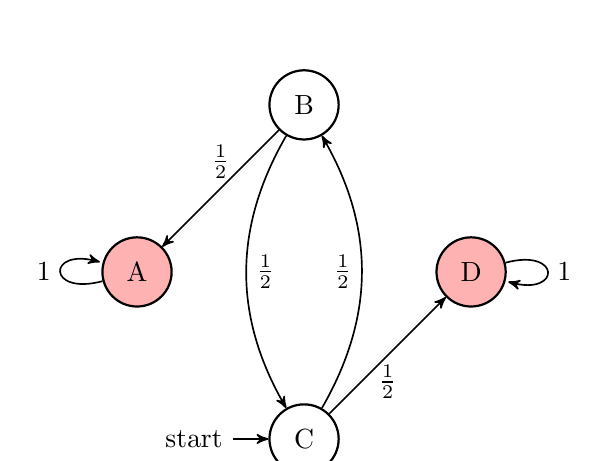
\begin{tikzpicture}[->,>=stealth',auto,semithick,node distance=3cm]
                \tikzstyle{every state}=[fill=white,draw=black,thick,text=black,scale=1]
                \node[state, fill=red!30]   (A)                     {A};
                \node[state]                (B)[above right of=A]   {B};
                \node[state, initial]       (C)[below right of=A]   {C};
                \node[state, fill=red!30]   (D)[above right of=C]   {D};

                \path
                (A) edge[loop left]     node{$1$}               (A)
                (B) edge[above]         node{$\frac{1}{2}$}     (A)
                edge[bend right]        node{$\frac{1}{2}$}     (C)
                (C) edge[below]         node{$\frac{1}{2}$}     (D)
                edge[bend right]        node{$\frac{1}{2}$}     (B)
                (D) edge[loop right]    node{$1$}               (D);
            \end{tikzpicture}
        \end{center}

        Given this chain, it's simply to write down a transition matrix
        \[
            P = \bordermatrix{
                & A & B & C & D         \cr
                A & 1 & 0 & 0 & 0       \cr
                B & 0.5 & 0 & 0.5 & 0   \cr
                C & 0 & 0.5 & 0.0 & 0.5 \cr
                D & 0 & 0 & 0 & 1
            }
        \]
    }
    \task{Which states are absorbing states?}
    {
        As it's shown on graph (with red color)
        and in transition matrix
        state A and D are absorbing.
    }
    \task{$P^{(n)}_{i,j}$ denotes the probability that a player starts with $i$ coins and then ends up with $j$
        coins in $n$ steps. Show that for an even number steps $(n)$ for a game where no player
        wins/loses that $P^{(n)}_{BB} = \rbra{\frac{1}{2}}^n $. Assume the same initial conditions given above.}
    {
        First of all, let's calculate two-step transition matrix:
        \[
            P^{(2)} = P^2 = \begin{pmatrix}
                1           & 0           & 0           & 0           \\
                \frac{1}{2} & \frac{1}{4} & 0           & \frac{1}{4} \\
                \frac{1}{4} & 0           & \frac{1}{2} & \frac{1}{2} \\
                0           & 0           & 0           & 1           \\
            \end{pmatrix}
        \]

        As we can see, in the second column only element corresponding to node B
        is not equal to 0, therefore for any $k \in \N$ we have $P^{2k}_{BB} = \frac{1}{4^k} = \rbra{\frac{1}{2}}^{2k} $.
        Then, for an even number $n = 2k$ we get: $P^{(n)}_{BB} = \rbra{\frac{1}{2}}^n$.
    }
\end{enumerate}

\section{Mouse house}
A mouse is in a maze with four cells (1 -- 4) and a path to freedom (cell 0) that can only
be reached from cell 4. The transition matrix of the mouse in the maze is given below with
indices from 0 -- 4 on each axis.
\[
    P = \bordermatrix{
        & 0 & 1 & 2 & 3 & 4 \cr
        0 & 1 & 0 & 0 & 0 & 0 \cr
        1 & 0 & 0 & \frac{1}{2} & \frac{1}{2} & 0 \cr
        2 & 0 & \frac{1}{2} & 0 & 0 & \frac{1}{2} \cr
        3 & 0 & \frac{1}{2} & 0 & 0 & \frac{1}{2} \cr
        4 & \frac{1}{3} & 0 & \frac{1}{3} & \frac{1}{3} & 0
    }
\]

\begin{enumerate}
    \task{Draw the maze using the information from the transition matrix.}
    {
        Instead of drawing maze we'd better to plot graph of markov
        chain corresponding this maze, because actually we just swap
        cells with states and doors with edges.
        \begin{center}
            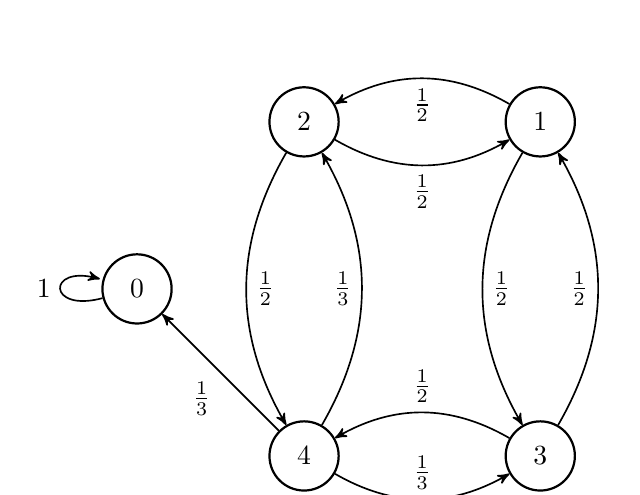
\begin{tikzpicture}[->,>=stealth',auto,semithick,node distance=3cm]
                \tikzstyle{every state}=[fill=white,draw=black,thick,text=black,scale=1]
                \node[state]    (A)                     {$0$};
                \node[state]    (C)[above right of=A]   {$2$};
                \node[state]    (B)[right of=C]         {$1$};
                \node[state]    (E)[below right of=A]   {$4$};
                \node[state]    (D)[right of=E]         {$3$};

                \path
                (A) edge[loop left]            node{$1$}               (A)
                (B) edge[bend right]           node{$\frac{1}{2}$}     (C)
                edge[bend right]               node{$\frac{1}{2}$}     (D)
                (C) edge[bend right, below]    node{$\frac{1}{2}$}     (B)
                edge[bend right]               node{$\frac{1}{2}$}     (E)
                (D) edge[bend right]           node{$\frac{1}{2}$}     (B)
                edge[bend right, above]        node{$\frac{1}{2}$}     (E)
                (E) edge[bend right]           node{$\frac{1}{3}$}     (C)
                edge[bend right]               node{$\frac{1}{3}$}     (D)
                edge                           node{$\frac{1}{3}$}     (A);
            \end{tikzpicture}
        \end{center}
    }
    \task{What is the probability that the mouse starts at 1 and then ends at 1 in two steps?}
    {
        In this task we have to calculate the following probability:
        \[
            P^{(2)}_{11} = P(x_2 = 1 | x_0 = 0)
        \]

        Applying the rule of total probability we get:
        \[
            P^{(2)}_{11} =
            \sum\limits_{k = 0}^{4} P(x_2 = 1 | x_1 = k,  x_0 = 1)
            P(x_1 = k | x_0 = 1)
        \]

        Finally, lets use markov property for the first element of
        each product and so we have:
        \[
            P^{(2)}_{11} =
            \sum\limits_{k = 0}^{4} P_{1k} P_{k1}
        \]

        Which equals to:
        \[
            P^{(2)}_{11} = 0 + 0 + \frac{1}{2} \cdot \frac{1}{2} + \frac{1}{2} \cdot \frac{1}{2} + 0 = \frac{1}{2}
        \]
    }
    \task{What is the 2-step transition matrix?}
    {
        Applying the same as in the previous subtask derivation for each combination of states,
        we get the following transition matrix:
        \[
            P^{(2)} = P^2 = \begin{pmatrix}
                1           & 0           & 0            & 0            & 0           \\
                0           & \frac{1}{2} & 0            & 0            & \frac{1}{2} \\
                \frac{1}{6} & 0           & \frac{5}{12} & \frac{5}{12} & 0           \\
                \frac{1}{6} & 0           & \frac{5}{12} & \frac{5}{12} & 0           \\
                \frac{1}{3} & \frac{1}{3} & 0            & 0            & \frac{1}{3} \\
            \end{pmatrix}
        \]
    }
\end{enumerate}

\section{Telephone calls}
The number of telephone calls arriving in a call center follows a Poisson process with a rate
of 1 phone call every 20 minutes $\rbra{\lambda = 3 \frac{1}{\text{hour}}}$.
What is the probability of getting at most
3 phone calls at time $[0, 1)$ (in hours), and then at least 4 phone calls at time $[1, 2)$, and
then at most 3 phone calls at time $[2, 3)$?

\sol{
    For compute the needed probability, let's calculate the probability
    for each subevent. So, for the first time range we,
    using property of Poisson process, get:
    \begin{align*}
        P(N(1) - N(0) \leq 3) \stackrel{N(0) = 0}{=}
        P(N(2) \leq 3) =
        \sum\limits_{k=0}^{3} \frac{\lambda^k}{k!} e^{-\lambda} & =           \\
        e^{-3} \rbra{ 1 + 3 + \frac{9}{2} + \frac{27}{6} }      & = 13 e^{-3}
    \end{align*}

    For the second time range we can use stationarity of
    increments: $N(t - s) \stackrel{d}{=} N(t) - N(s)$
    \[
        P(N(2) - N(1) \geq 4) \stackrel{stat. incr.}{=}
        P(N(1) \geq 4) = 1 - P(N(1) \leq 3) = 1 - 13 e^{-3}
    \]

    And for the last time range:
    \[
        P(N(3) - N(2) \leq 3) \stackrel{stat. incr.}{=}
        P(N(1) \leq 3) = 13 e^{-3}
    \]

    Now, we can compute the asked probability as multiplication of
    this 3 result, because Poisson process has independent increments:
    \[
        P(N(1) - N(0) \leq 3, N(2) - N(1) \geq 4, N(3) - N(2) \leq 3) =
        13^2 e^{6} (1 - 13 e^{-3})
    \]
}

\section{Chapman-Kolmogorov}
A Markov chain has the transition probability matrix given below. What is the 2-step transition probability
$P^{(2)}_{0,2}$? Solve this problem two ways by using the Chapman-Kolmogorov
equation and by calculating the 2-step transition matrix.

\[
    P = \bordermatrix{
        & 0 & 1 & 2 \cr
        0 & 0.6 & 0.3 & 0.1  \cr
        1 & 0.2 & 0.5 & 0.3 \cr
        2 & 0.4 & 0.4 & 0.2
    }
\]

\sol{
    The Chapman-Kolmogorov equation claims that
    \[
        P^{(n+m)}_{ij} =
        \sum\limits_{k=1}^{K} P^{(n)}_{ik} P^{(m)}_{kj}
    \]

    Then, we get
    \[
        P^{(1+1)}_{0,2} =
        \sum\limits_{k=1}^{K} P_{0k} P_{k2} = 0.17
    \]

    Actually the same, we do when derive $n$-step transition matrix, so
    in this case $P^{(1+1)}_{0,2}$ is equal to $(0,2)$ element of the
    following matrix:
    \[
        P^{(2)} = P^2 = \begin{pmatrix}
            0.46 & 0.37 & 0.17 \\
            0.34 & 0.43 & 0.23 \\
            0.4  & 0.4  & 0.2  \\
        \end{pmatrix}
    \]
}

\section{Drunk friends}
Your three drunk friends (A, B, and C) are walking back home from a party in your
house. Because two of them (A and B) live together, you tie their hands together. One
hour later, you discover that none of them have reached their homes! Assume that each
person independently chooses to walk in a random direction (north, south, east, or west)
at a rate of 1 step per second, and that A and B will only move if they agree on the direction:
\begin{enumerate}
    \task{Simulate 500 possible trajectories of A (and B) and C after 1 hour.
        Plot the distributions of the distance from your house.}
    {
        From the simulation during 3600 seconds
        we've retriever 500 distances from
        the center. The histogram of these data is shown below. As we can
        see, linkage between A and B leads to significantly lower
        result distance than it is for C.

        \begin{figure}[!ht]
            \begin{subfigure}{.5\textwidth}
                \begin{tikzpicture}
                    \begin{axis}[ybar, ymin=0]
                        \addplot +[hist={bins=10}] table [y index=0] {distAB.csv};
                    \end{axis}
                \end{tikzpicture}
                \caption{Histogram of the distance to the A (and B)}
            \end{subfigure}
            \begin{subfigure}{.5\textwidth}
                \begin{tikzpicture}
                    \begin{axis}[ybar, ymin=0]
                        \addplot +[hist={bins=10}] table [y index=0] {distC.csv};
                    \end{axis}
                \end{tikzpicture}
                \caption{Histogram of the distance to the C}
            \end{subfigure}
        \end{figure}
        \pagebreak
    }
    \task{From the results of your simulation, how far away from your house should you search
        for A (and B) and C to have a 60\% chance of finding each of them?}
    {
        From the simulated data a 60\% chance of finding A (and B) or C
        is possible to calculate as a $0.6$ quantile. Thus, for
        our data it is $\approx 28.38$ and $\approx 57.82$ for A (with B) and C respectively.
    }
\end{enumerate}

\end{document}